\documentclass[border=5pt]{standalone}
\usepackage{pgfplots}
\pgfplotsset{compat=1.18}
\begin{document}
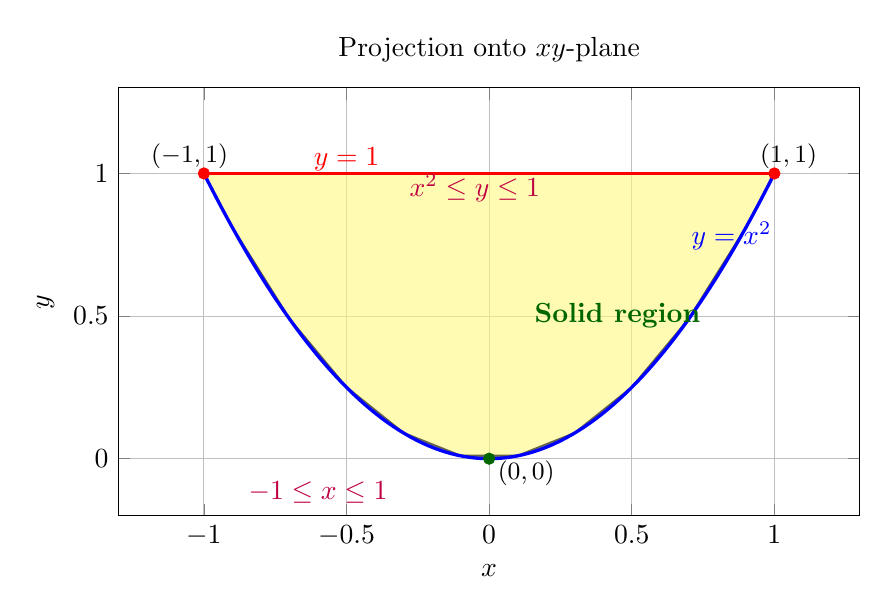
\begin{tikzpicture}
\begin{axis}[
    title={Projection onto $xy$-plane},
    xlabel={$x$}, ylabel={$y$},
    xmin=-1.3, xmax=1.3,
    ymin=-0.2, ymax=1.3,
    axis equal image,
    grid=both,
    width=11cm, height=11cm,
]

% Shade region: x^2 <= y <= 1
\addplot[draw=black, fill=yellow!50, opacity=0.6, thick] coordinates {
    (-1, 1) (1, 1) (0.9, 0.81) (0.7, 0.49) (0.5, 0.25) (0.3, 0.09) (0.1, 0.01)
    (-0.1, 0.01) (-0.3, 0.09) (-0.5, 0.25) (-0.7, 0.49) (-0.9, 0.81) (-1, 1)
};

% Parabola y = x^2
\addplot[blue, very thick, domain=-1:1, samples=100] {x^2};

% Line y = 1
\addplot[red, very thick, domain=-1:1] {1};

% Annotations
\node[blue] at (axis cs:0.85, 0.78) {$y=x^2$};
\node[red] at (axis cs:-0.5, 1.05) {$y=1$};
\node[green!40!black, font=\bfseries] at (axis cs:0.45, 0.5) {Solid region};
\node[purple] at (axis cs:-0.05, 0.95) {$x^2 \le y \le 1$};
\node[purple] at (axis cs:-0.6, -0.12) {$-1 \le x \le 1$};

% Mark key points
\addplot[only marks, mark=*, mark size=2pt, color=red] coordinates {(-1,1) (1,1)};
\addplot[only marks, mark=*, mark size=2pt, color=green!40!black] coordinates {(0,0)};
\node[font=\small] at (axis cs:1.05, 1.06) {$(1,1)$};
\node[font=\small] at (axis cs:-1.05, 1.06) {$(-1,1)$};
\node[font=\small] at (axis cs:0.13, -0.05) {$(0,0)$};

\end{axis}
\end{tikzpicture}
\end{document}